\chapter{專題}

\section{翻譯專題}
\subsection{正確翻譯被動語態}
\begin{itemize}
  \itemsep0em
  \item He was laughed \hilight{at} by his friends. 他受到了朋友的嘲笑.
  \item Our foreign policy is supported by people all over the world. 我國的外交政策得到了全世界人民的支持.
  \item These questions will be discussed briefly. 這些問題將予以簡單討論.
  \item The boy was criticised yesterday. 這孩子昨天挨了一頓批.
  \item A police court is presided over by a magistrate, who tries the cases without a jury. 治安法庭由地方法官主持, 法官審理各種案件, 無須陪審團.
\end{itemize}

\subsection{正確翻譯過去式強調句型}
\begin{multicols}{2}
\begin{itemize}
  \itemsep0em
  \item It is generally accepted that: 普遍認為
  \item It is believed that: 據信
  \item It is well known that: 眾所周知
  \item It is learned that: 據悉
  \item It is estimated that: 據估計
  \item It must be pointed out that: 必須指出
  \item It is understood that: 不用說
  \item It cannot be denied that: 無可否認
  \item It has been proved that: 已經證明
  \item It may be confirmed that: 可以肯定
  \item It may be safely said that: 可以有把握地說
  \item It is sometimes asked that: 人們有時會問
  \item It is expected that: 人們希望
  \item It is said that: 據說
  \item It is reported that: 據報道
\end{itemize}
\end{multicols}

\section{詞彙專題}
\subsection{Medicare (國民醫療保健)}
\begin{itemize}
  \itemsep0em
  \item Medicare: 國民醫療保健
  \item Bulk Bill: 刷Medicare卡公費醫療
  \item public / private patient: 公費醫療保險 / 私人醫療保險的病人
  \item Child Support: \hilight{子女撫養費}
  \item in patient / out patient: 住院病人 / 門診病人
  \item Pharmaceutical Benefits Scheme (PBS): 藥物補助計劃
  \item Repatriation Pharmaceutical Benefits Scheme: 退伍軍人藥物補助計劃
  \item Health Care Card: 健康醫療保健卡 (一般用於低收入或上年紀的人)
  \item PBS Safety Nets: 藥物補助計劃安全網 (檢查哪些藥物項目被cover)
  \item Teen Dental: 青少年牙科服務
  \item Make a Claim: 報銷申請
  \item Commonwealth Seniors Health Card: 聯邦老年保健卡
  \item Office of Hearing Services: 聽力服務處
  \item Medicare Benefit Tax Statement: 國民醫療保健稅務報告
  \item Medicare Benefits Schedule (MBS): 國民醫療保健福利計劃
  \item Medicare Levy Exemption: 國民醫療保健豁免
  \item Health Identifiers Service: 醫療保健尋找服務 (適用於偏遠地區的人)
  \item \hilight{Cleft Lip} and \hilight{Cleft Palate Scheme}: 唇齶裂畸形計劃
  \item Australian Government Department of Human Service: 澳洲\hilight{民政部}
\end{itemize}

\subsection{正確表示地點(重點)}
\begin{itemize}
  \itemsep0em
  \item at 可以單接unit, 也接具體的完整的地址, 注意英漢翻譯的時候地址從小到大顛倒!
  \item on 或 in 單接street / road
  \item in 單接suburb
  \item Arrived \hilight{in} Sydney / Arrived \hilight{at} Sydney airport.
\end{itemize}

\subsection{和學校有關的詞}
\begin{multicols}{2}
\begin{itemize}
  \itemsep0em
  \item \textbf{關於職位和人}:
  \begin{enumerate}
    \itemsep0em
    \item 班主任: head teacher
    \item 校長: principal / headmaster
    \item 心理咨詢師: counsellor
    \item 職業顧問: career advisor (中學里可用於幫助學生選課)
    \item 校醫: school nurse
    \item 教練: coach
  \end{enumerate}
  \item \textbf{中國特有的學歷}:
  \begin{enumerate}
    \itemsep0em
    \item 中專: Technical Secondary School
    \item 職高: Vocational Secondary School
    \item 大專: Junior College
  \end{enumerate}
  \item \textbf{不同的學生}:
  \begin{enumerate}
    \itemsep0em
    \item 寄宿 / 走讀生: boarding / day student
    \item 小學生: pupil
  \end{enumerate}
\end{itemize}
\end{multicols}

\subsection{和保險有關的詞}
\begin{multicols}{2}
\begin{itemize}
  \itemsep0em
  \item 第三方強制險: CTP (Compulsory Third Party Insurance)
  \item 綠單子: Green Slip\footnote{CTP Green Slip (NSW). Green Slip或者Compulsory Third Party insurance稱為第三方基本保險,是一種強制執行的\\汽車保險。}
  \item 建築物與屋內財產的保險: Home buildings / Home contents
  \item 收入保障: Income Protection
  \item 保單號: Policy Number
  \item 保費: premium
  \item 墊底費\footnote{墊底費,實際上是國際上大多數財產保險類公司對投保人進行理賠的時候收取損失「均攤」費用的一種通行做法。當保險\\投保人由於疏忽或是無可抗拒的力量,產生了財產損失並向保險公司進行索賠的時候,需要先為自己的過失 \\ 造成的損失進行費用墊付;所以,Excess Fee才被稱作「墊底費」或是「打底費」,英文也稱作Deductible。}: excess fee
\end{itemize}
\end{multicols}

\subsection{和毒品有關的詞}
\begin{multicols}{2}
\begin{itemize}
  \itemsep0em
  \item ecstasy: 迷幻劑
  \item heroin: 海洛因
  \item ice: 病毒
  \item marihuana (cannabis): 大麻
  \item cocaine: 可卡因
  \item morphine: 嗎啡
  \item caffeine: 咖啡因
\end{itemize}
\end{multicols}

\subsection{和竞拍有關的詞}
\begin{multicols}{2}
\begin{itemize}
  \itemsep0em
  \item 竞价: bid, bidding
  \item 参加竞拍的人: bidder
  \item 起拍价: starting price / open bidding
  \item 成交价: hammer price / winning bid
  \item 抬高价格: bid up the price
\end{itemize}
\end{multicols}

\subsection{澳洲移民相關簽證}
\begin{itemize}
  \itemsep0em
  \item Independent Skilled Migration Scheme: 獨立技術移民方案
  \item General Skilled Migration Scheme: 一般技術移民方案
  \item Spouse / Parent Migration Scheme: 配偶 / 父母移民方案
  \item Employer / State-Government Sponsored Scheme: 雇主 / 州政府擔保方案
  \item Regional Area Sponsored Scheme: 偏遠地區擔保方案
  \item ENSOL (Employer Nomination Skill Occupation List): 雇主提名技術職業列表
  \item Visitor's Visa: 訪客簽證
  \item tourist / visitor's / student / business / working holiday (打工度假)
  \item parent / spouse / temporary skilled graduate
  \item prospective marriage visa: 預期婚姻簽證 (也叫fianc$\acute{e}$ visa: 未婚夫妻簽證)
  \item PSW (Post Study Working visa)
\end{itemize}

\subsection{和藍領職業有關的詞}
\begin{multicols}{2}
\begin{itemize}
  \itemsep0em
  \item 電工: electrician
  \item 水管工: plumber (b不發音)
  \item 木工: carpenter
  \item 石膏板(牆)工: gyprocker
  \item 磚工: bricklayer
  \item 瓷磚工: tiler
  \item (泛指)建築工人 / 承建商: builder
  \item 護工(有別於護士): nurse aid / assistant
  \item 教會醫院的護士: sister
\end{itemize}
\end{multicols}

\subsection{和銀行有關的詞}
\begin{itemize}
  \itemsep0em
  \item 西太銀行: WestPac
  \item 國民銀行: NAB (National Australia Bank)
  \item 聯邦銀行: Commonwealth Bank
  \item 澳新銀行: ANZ (Australia and New Zealand Banking Group)
\end{itemize}

\subsection{宣傳冊和傳單}
\begin{itemize}
  \itemsep0em
  \item 小冊子(裝訂成冊): booklet / pamphlet / brochure
  \item 單頁傳單: flyer / leaflet
  \item 彩頁的: colour-printed
\end{itemize}

\subsection{和不同類型的房子}
\begin{multicols}{2}
\begin{itemize}
  \itemsep0em
  \item \hilight{獨棟屋: house}
  \begin{center}
    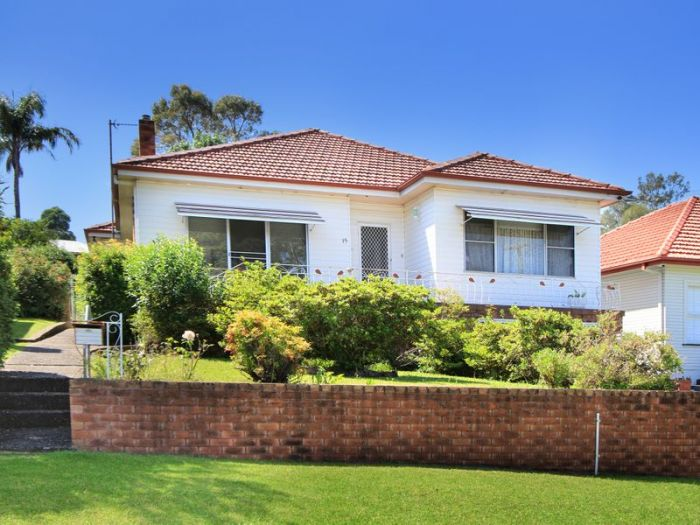
\includegraphics[scale=0.4]{pics/house}
  \end{center}
  \item 連排屋(多層): town house
  \begin{center}
    
\includegraphics[scale=0.3]{pics/townhouse}
  \end{center}
  \item 後院加蓋屋 / 祖母房: granny flat
  \begin{center}
    
\includegraphics[scale=0.3]{pics/granny-flat}
  \end{center}
  \item \hilight{小套間: studio}
  \item 公寓: apartment
  \item 單元房: unit
\end{itemize}
\end{multicols}

\subsection{不同的救助補貼}
\begin{itemize}
  \itemsep0em
  \item 失業補貼: Unemployment allowance / benefit
  \item 新開始津貼: Newstart allowance\footnote{為那些正在尋找工作的人士提供的輔助收入。您需要符合下列條件才能申請:年齡20以上。失業但是能夠工作,同時\\也在積極找工;另外已經在就近的 Centrelink 辦事處註冊登記。}
  \item 青年津貼(小於25歲): Youth allowance\footnote{為青年提供的一項新的津貼。在生病、尋工、學習或接受訓練期間,您都可以申請領取這項福利。}
\end{itemize}

\subsection{那些我已讀錯好多年的單詞}
\begin{multicols}{3}
\begin{itemize}
  \itemsep0em
  \item months
  \item divorce
  \item parole / patrol
  \item sedative
  \item indigestion
  \item gaol
  \item deteriorate
  \item debts
  \item plumber
  \item sham
  \item whooping
  \item diarrhoea
  \item depot
\end{itemize}
\end{multicols}

\section{道德題}
\subsection{澳大利亞公眾假日}
\begin{itemize}
  \itemsep0em
  \item Australia Day: 26 January
  \item Royal Hobart Regatta: 2nd Monday in February
  \item Labour Day: 1st Monday in March
  \item Western Australia Day: 1st Monday in June
  \item Labour Day: 1st Monday in October
  \item Canberra Day: 2nd Monday in March
\end{itemize}

\subsection{犯人被捕程序}
建議暫時參考: \url{https://www.lawsociety.com.au/community/publicationsandfaqs/UnderArrest/index.htm}

\url{http://www.lawhandbook.sa.gov.au/ch03s01s03s01.php}